\section{Cursograma Producci\'on}
\begin{center}
 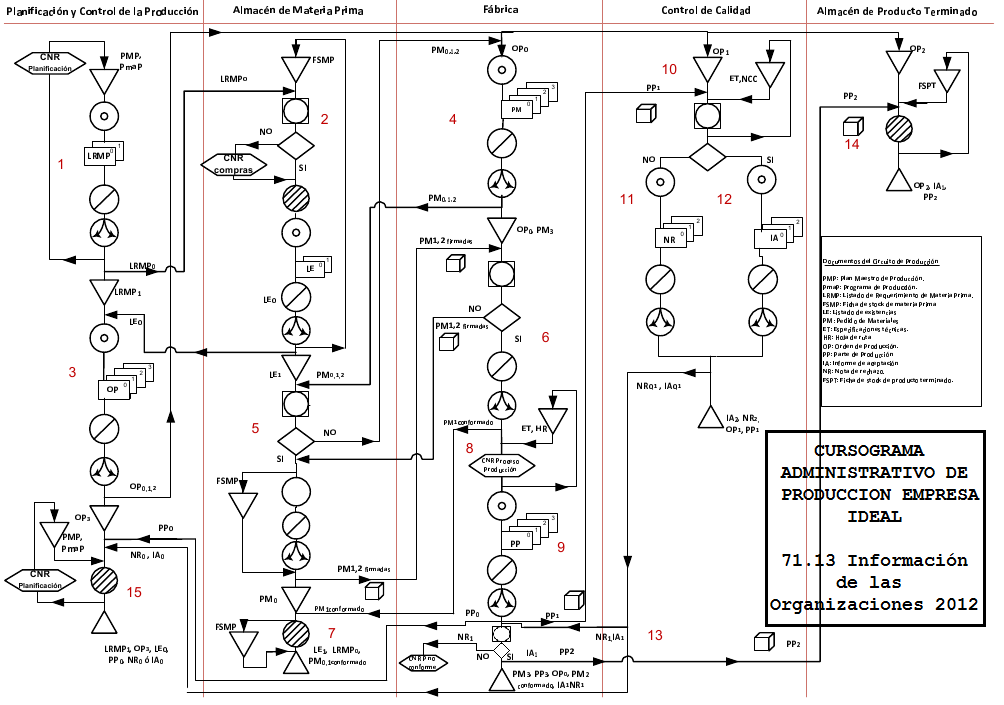
\includegraphics[angle=90,scale=0.95,keepaspectratio=true]{./Circuitos-Teoricos/Produccion/Images/cursograma-produccion.png}
 % cursograma-produccion.png: 1004x705 pixel, 96dpi, 26.56x18.65 cm, bb=0 0 753 529
\end{center}

\section{Procedimiento de Producci\'on}
\begin{center}
 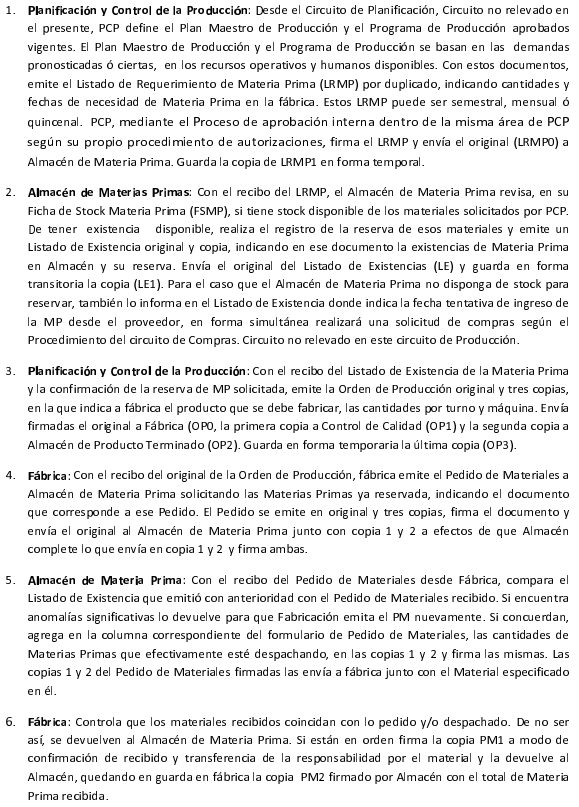
\includegraphics[keepaspectratio=true]{./Circuitos-Teoricos/Produccion/Images/procedimiento-produccion.png}
 % procedimiento-produccion.png: 579x807 pixel, 96dpi, 15.32x21.35 cm, bb=0 0 434 605
\end{center}
\begin{center}
 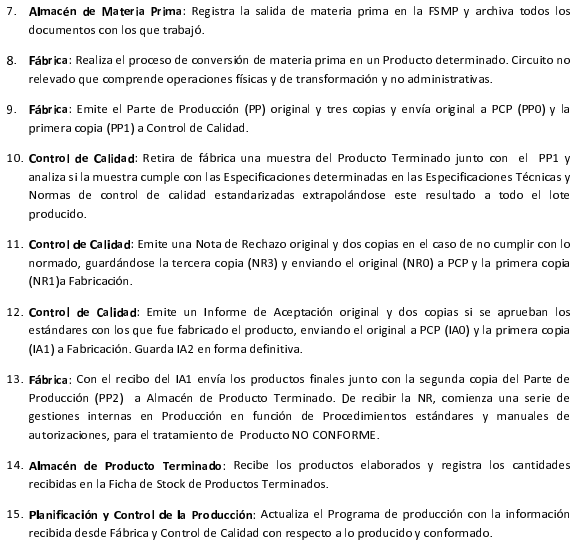
\includegraphics{./Circuitos-Teoricos/Produccion/Images/procedimiento-produccion-2.png}
 % procedimiento-produccion-2.png: 576x545 pixel, 96dpi, 15.24x14.42 cm, bb=0 0 432 409
\end{center}

\pagebreak
\section{Cursograma de Producci\'on (con numeración para el manual)}
\subsection{Manual del Cursograma de Producci\'on}

\begin{center}\textbf{Sectores intervinientes}\end{center}
\begin{itemize}
  \item Planificaci\'on y Control de Producci\'on
  \item Almac\'en de Materia Prima
  \item F\'abrica
  \item Control de Calidad
  \item Almac\'en de Producto Terminado
\end{itemize}

\emph{\textbf{TODO}}

\pagebreak
\section{Formularios de Producci\'on}

\subsection{Orden de Producci\'on}
\begin{center}
 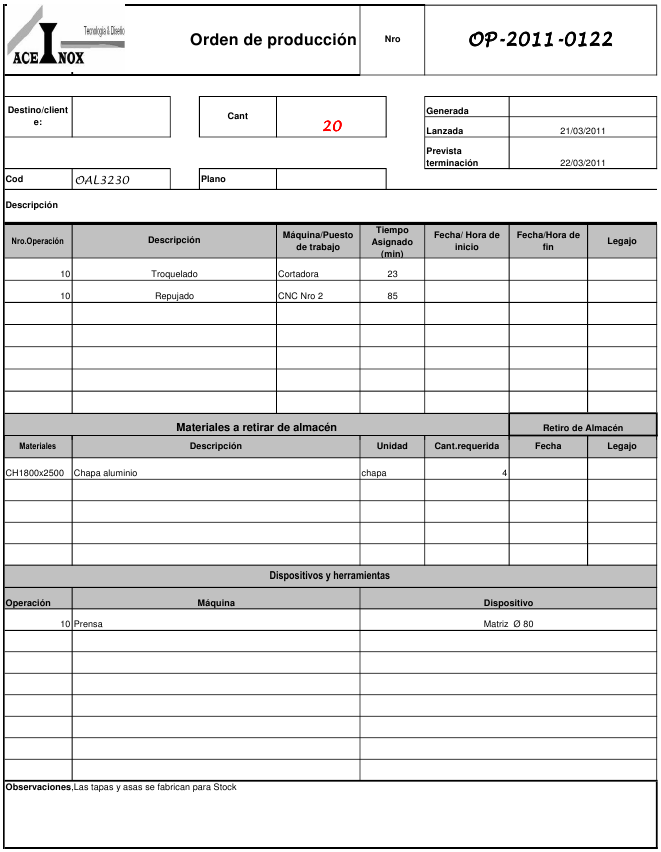
\includegraphics[scale=0.9,keepaspectratio=true]{./Circuitos-Teoricos/Produccion/Images/orden-de-produccion.png}
 % orden-de-produccion.png: 661x852 pixel, 96dpi, 17.49x22.54 cm, bb=0 0 496 639
\end{center}

\subsubsection{Descripción}
\emph{\textbf{TODO}}

\pagebreak
\subsection{Hoja de Ruta}
\begin{center}
 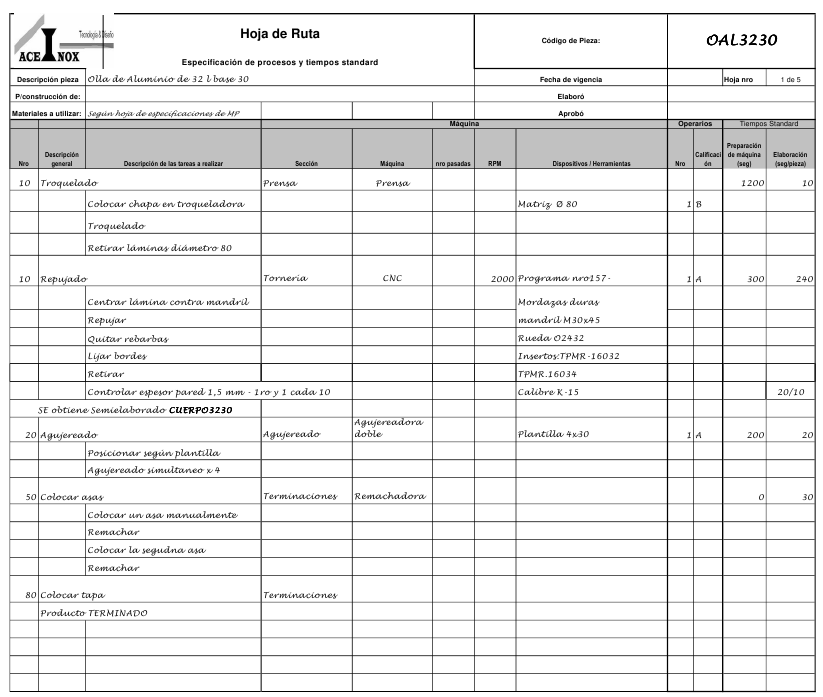
\includegraphics[angle=90,scale=0.95,keepaspectratio=true]{./Circuitos-Teoricos/Produccion/Images/hoja-de-ruta.png}
 % hoja-de-ruta.png: 823x697 pixel, 96dpi, 21.77x18.44 cm, bb=0 0 617 523
\end{center}

\subsubsection{Descripción}
\emph{\textbf{TODO}}

\pagebreak
\section{Normas de control interno generales y específicas de Producci\'on}
\emph{\textbf{TODO}}

\subsection{Normas Específicas}
\emph{\textbf{TODO}}
